\subsubsection{Virkemåte}
Pensum I fys1210 er å kunne beskrive hvordan et batteri fungerer.
\\

Batterier deles i to grupper: oppladbare batterier og engangsbatterier.
I fys1210 skal vi se nærmere på engangbatterier.

Det finnes mange typer engangsbatterier som blant annet:
Sink-karbon batterier, alkaliske batterier og lithium batterier.
Men de fleste batteriene er bygget realtivit likt:
\\

Et batteri består av to elektroder,
en anode som er negativ ladet og en katode som er postiv ladet.
I tillegg har batteriet en elektrolytt som skiller disse fra hverandre.
Dette er ofte en væske eller gele som kun leder ioner, men ikke elektroner.

Når man da kobler noe til batteriet, f.eks. en diode,
slik at det blir en lukket krets
så vil det oppstå en kjemisk reakjson
der elektroner fra anoden beveger seg over til katoden.
Akkurat som vist på tegningen.
\\
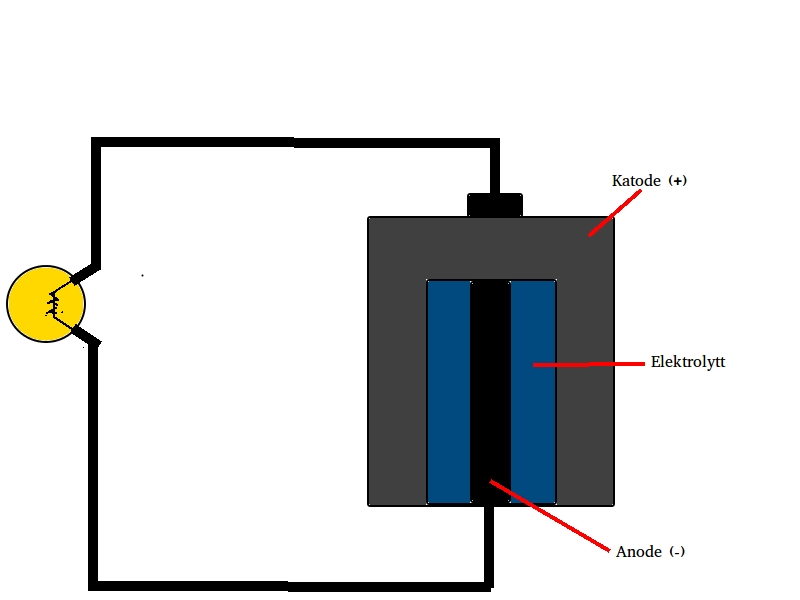
\includegraphics[width=\textwidth]{./img/batteri}

\subsubsection{Maksimal effektoverføring}
\paragraph{Ideell spenningskilde} \mbox{} \\
En perfekt spenningskilde vil ha like stor spenning hele tiden,
uavhengig av hvor mye strøm den leverer.
I virkeligheten vil dette ikke være sant for en reell spenningskilde.
\\\\
Strømmen ut av en spenningskilde vil påvirkes av kildens indre motstand
(tenk thevenin).
Eksempel på indre motstand: \\
Lommelyktbatteri: 1 til 10 \SI{}{\ohm}. \\
Bilbatteri: 0.01 til 0.004 \SI{}{\ohm}.



\paragraph{Maximum power!} \mbox{} \\
Effekten $P$ fra en spenningskilde maksimaliseres når man kobler på
en lastmotstand som er \emph{lik} kildens indre motstand.
$$R_L = R_I$$
Effekt er gitt ved ligningen
$$P = \frac{U^2}{R}$$


\subsubsection{Motstand og temperatur}
TODO

